%%% Template originaly created by Karol Kozioł (mail@karol-koziol.net) and modified for ShareLaTeX use

\documentclass[a4paper,fleqn,11pt]{article}

\usepackage[T1]{fontenc}
\usepackage[utf8]{inputenc}
\usepackage{graphicx}
\usepackage{xcolor}

\usepackage{tgtermes}

\usepackage[
pdftitle={EE698G - Probabilistic Mobile Robotics Assignment}, 
pdfauthor={Satya Prakash Panuganti, 14610},
colorlinks=true,linkcolor=blue,urlcolor=blue,citecolor=blue,bookmarks=true,
bookmarksopenlevel=2]{hyperref}
\usepackage{amsmath,amssymb,amsthm,textcomp}
\usepackage{enumerate}
\usepackage{multicol}
\usepackage{tikz}

\usepackage{geometry}
\geometry{total={210mm,297mm},
left=15mm,right=15mm,%
bindingoffset=0mm, top=15mm,bottom=15mm}

\usepackage{ mathrsfs }
\usepackage{ mathtools }

\linespread{1.3}

\newcommand{\linia}{\rule{\linewidth}{0.5pt}}

% custom theorems if needed
\newtheoremstyle{mytheor}
    {1ex}{1ex}{\normalfont}{0pt}{\scshape}{.}{1ex}
    {{\thmname{#1 }}{\thmnumber{#2}}{\thmnote{ (#3)}}}

\theoremstyle{mytheor}
\newtheorem{defi}{Definition}

% my own titles
\makeatletter
\renewcommand{\maketitle}{
\begin{center}
\vspace{2ex}
{\huge \textsc{\@title}}
\vspace{1ex}
\\
\linia\\
\@author \hfill \@date
\vspace{4ex}
\end{center}
}
\makeatother
%%%

% custom footers and headers
\usepackage{fancyhdr,lastpage}
\pagestyle{fancy}
\lhead{}
\chead{}
\rhead{}
\lfoot{Assignment 1}
\cfoot{}
\rfoot{Page \thepage\ /\ \pageref*{LastPage}}
\renewcommand{\headrulewidth}{0pt}
\renewcommand{\footrulewidth}{0pt}
%

%%%----------%%%----------%%%----------%%%----------%%%

\begin{document}

\title{EE604A - Digital Image Processing Assignment}

\author{Satya Prakash Panuganti, 14610}

\date{1 September, 2017}

\maketitle

\section*{Image Sources}
Sunset  (high.jpg)  : \url{https://www.flickr.com/photos/mediaflex/4190084346} \\
Carving (low.jpg)   : \url{https://www.flickr.com/photos/30440933@N06/2847993403} \\
Dog     (small.jpg) : \url{https://res.cloudinary.com/rover-com/image/upload/a_exif,c_fill,f_jpg,fl_progressive,g_face:center,h_100,q_80,w_100/remote/images/pets/4NpPzO8N/50e4a023d9/original.jpg} \\
Face (divyat.jpg)   : Own work. Taken with permission.
\section*{Solution 1}
\subsection*{(a)}
Code has been written in three MATLAB\textregistered  files :
\begin{itemize}
\item Q1/lloyd\_max\_quantizer\_function.m : The file containing the function which retruns the mean square errors, representation levels and transition levels given the pdf of a signal.
\item normal.m : File containing function which returns the pdf value at a point.
\item Q1/Q1.m : The script to perform the required tasks.
\end{itemize}
\subsection*{(b)}
The Lloyd-Max Quantizer was run over a signal with zero mean and unit variance normal distribution.
The 4 representation levels are : -1.5104  -0.4528  0.4528  1.5104 \\
The corresponding transition levels are : $-\infty$  -0.9816  0.0000  0.9816  $\infty$
\subsection*{(c)}
\begin{center}
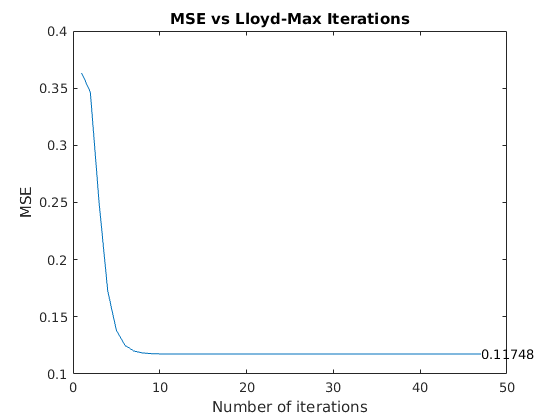
\includegraphics[scale=0.70]{../results/lloyd.png}
\end{center}
\subsection*{(d)}
\subsubsection*{Experiments}
In all of the experiments, the transition levels were intialy choosen uniformaly between -10 and 10. The smallest and largest transition levels were than forced to $-\infty$ and $\infty$ respectively. \\
\begin{tabular}{| c | c | c | c | c | c | c | c | c | c | c | c |}
	\hline
	$\mu$ &	$\sigma^2$ &$l_1$ &		$l_2$ &		$l_3$ &		$l_4$ &		$m_1$ &		$m_2$ &			$m_3$ &		$m_4$ &		$m_5$ &		MSE \\
	\hline
	0 &		1 &			-1.5104 &	-0.4528 &	0.4528 &	1.5104 &	$-\infty$ &	-0.9816 &	0.0000 &	0.9816 &	$\infty$ &	0.11748 \\
	\hline
	0 &		0.5 &		-1.0680 &	-0.3202 &	0.3202 &	1.0680 &	$-\infty$ &	-0.6941 &	0.0000 &	0.6941 &	$\infty$ &	0.041536 \\
	\hline
	0 &		2 &			-2.1361 &  	-0.6403 & 	0.6403 & 	2.1361 &	$-\infty$ &	-1.3882 &	0.0000 &	1.3882 &	$\infty$ &	0.33229 \\
	\hline
	2.3 &   1 &			0.7896 &	1.8472 &	2.7528 &	3.8104 &	$-\infty$ &	1.3184 &	2.3000 &	3.2816 &	$\infty$ &	0.11748 \\
	\hline
	2.3 &	0.5 &		1.2320 &	1.9798 &	2.6202 &	3.3680 &	$-\infty$ &	1.6059 &	2.3000 &	2.9941 &	$\infty$ &	0.041536 \\
	\hline
	2.3 &	2 &			0.1639 &	1.6597 & 	2.9403 &	4.4361 &	$-\infty$ &	0.9118 &	2.3000 &	3.6882 &	$\infty$ &	0.33229 \\
	\hline
\end{tabular}
\subsubsection*{Observations}
\begin{enumerate}
\item On adding a $\Delta\mu$ to the mean, while keeping $\sigma^2$ constant, the representation and transition levels obatined get shifted by $\Delta\mu$ as well.
\item The MSE value are independent of the mean.
\item As $\sigma \uparrow$, MSE $\uparrow$ and $|l_{i + 1} - l_i| \uparrow$
\end{enumerate}

\subsection*{(e)}
Let the signal be given by $S$ and the pdf of $S$ be $p_S (s)$.
\begin{align*}
Now,\ p_S (s) = \begin{dcases*}
					\frac{1}{b - a}	& $a \leq s < b$\\
					0  				& otherwise
				\end{dcases*}
\end{align*}
Let us assume that there `L' representation levels, $a_i$ be the representation levels and $m_i$ be the transition levels. \\
We begin by initializing $m_i$ uniformly :
\begin{align*}
m_i = a + \frac{b - a}{L} \times (i - 1)\ \forall\ i \in [1, L + 1]
\end{align*}
We next set $a_i$ :
\begin{align*}
a_i &  = \frac{\int_{m_i}^{m_{i + 1}} s \times p_S (s) ds}{\int_{m_i}^{m_{i + 1}} p_S (s) ds}\ \forall\ i \in [1, L] \\
    & = \frac{\frac{m_{i + 1}^2 - {m_i}^2}{2(b - a)}}{\frac{m_{i + 1} - {m_i}}{b - a}}\ \forall\ i \in [1, L] \\
    & = \frac{m_i + m_{i + 1}}{2}\ \forall\ i \in [1, L] \\
    & = a + \frac{b - a}{L} \times \frac{i + i - 1}{2}\ \forall\ i \in [1, L] \\
    & = a + \frac{(b - a)(2i - 1)}{2L}\ \forall\ i \in [1, L]
\end{align*}
We now set $m_i$ :
\begin{align*}
m_i & = \frac{a_{i - 1} + a_i}{2}\ \forall\ i \in [2, L] \\
	& = a + \frac{b - a}{4L} \times (2 (i + i - 1) - 2)\ \forall\ i \in [2, L] \\
	& = a + \frac{b - a}{L} \times (i - 1)\ \forall\ i \in [2, L]
\end{align*}
$m_i$ do not change in the above step. Hence, the Lloyd-Max Quantizer has converged to a final solution.

\section*{Solution 2}
A C++ function, EE604A::histogram\_matching(), for histogram matching of cv::Mat images has been developed.
The code required for the matching function is present in :
\begin{itemize}
\item Q2/src/histogram\_matching.cxx
\item Q2/src/histogram\_matching.h 
\end{itemize}
A small program which uses the histogram matching function is present in Q2/src/Q2.cxx

In order to build and run the code, the following steps need to be followed :
\begin{enumerate}
\item Enter Q2/src through terminal.
\item run build.sh (OpenCV needs to installed and a version of g++ supporting c++14 needs to be present)
\item Execute Q2 (the binary file) with the reference and target relative/absolute image paths. Eg. [./Q2 ../../images/high.jpg ../../images/low.jpg] or [./Q2 ../../images/low.jpg ../../images/high.jpg] (On Ubuntu)
\item The program can be closed by Ctrl+C on the terminal or by pressing `q' when one of the image windows is open.
\end{enumerate}
REMARK : A simple plot of the the histograms can be obtained on the terminal by toggling the third argument of the function EE604A::histogram\_matching() to true.

\pagebreak

\subsection*{Results}
\begin{center}
Target : high.jpg, Reference : low.jpg \\
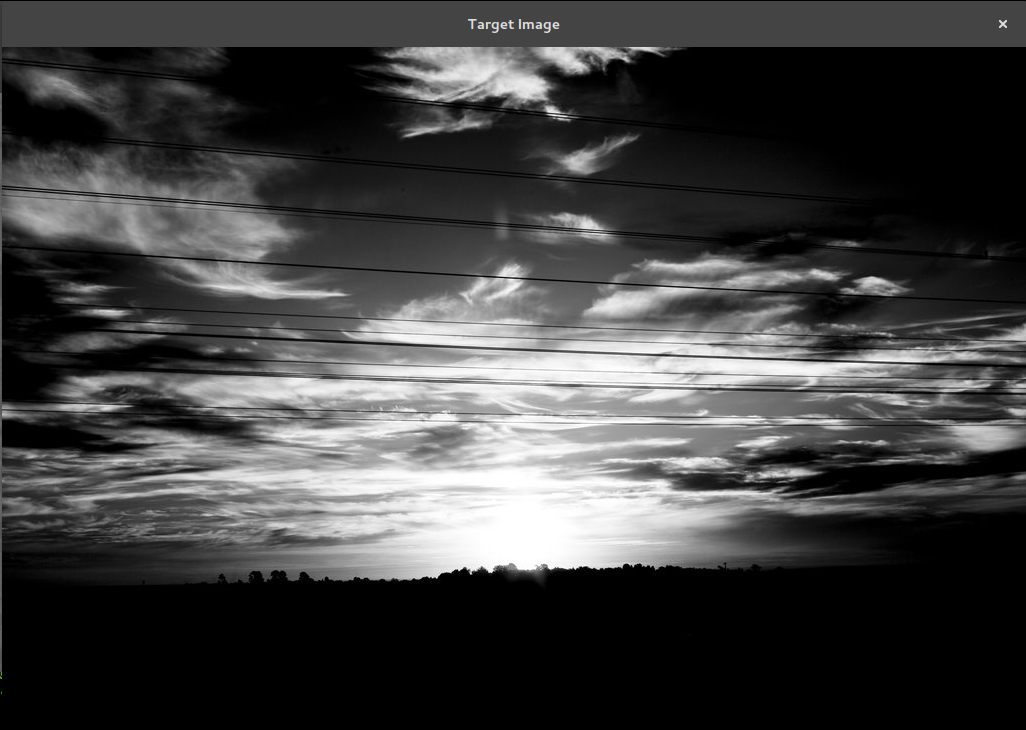
\includegraphics[scale=0.28]{../results/target1.png}
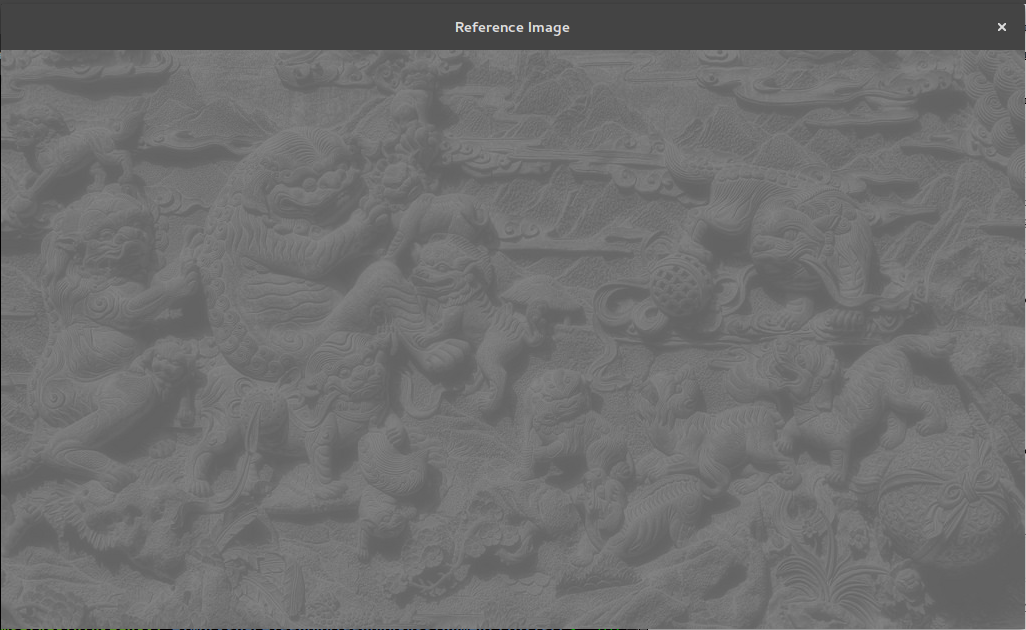
\includegraphics[scale=0.28]{../results/reference1.png}
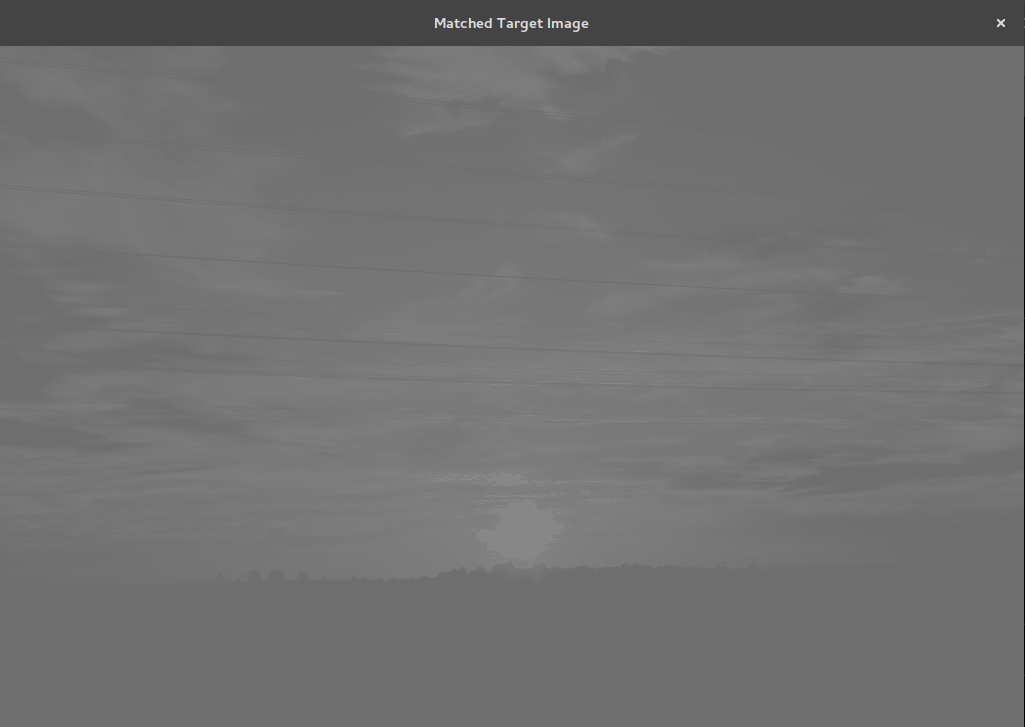
\includegraphics[scale=0.28]{../results/matched1.png}
\end{center}

\pagebreak

\begin{center}
Target : low.jpg, Reference : high.jpg \\
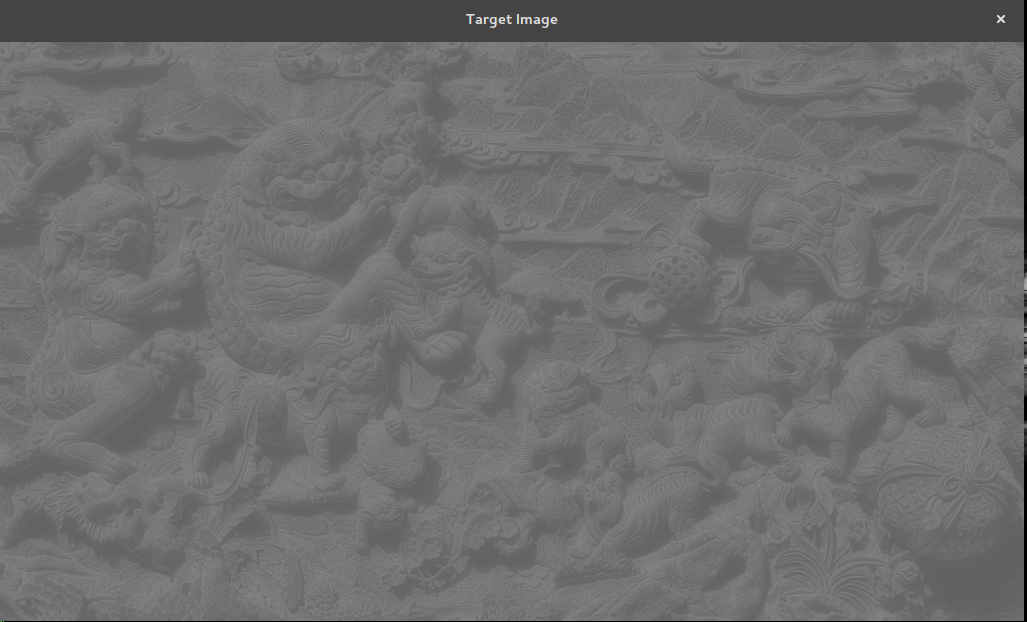
\includegraphics[scale=0.28]{../results/target2.png}
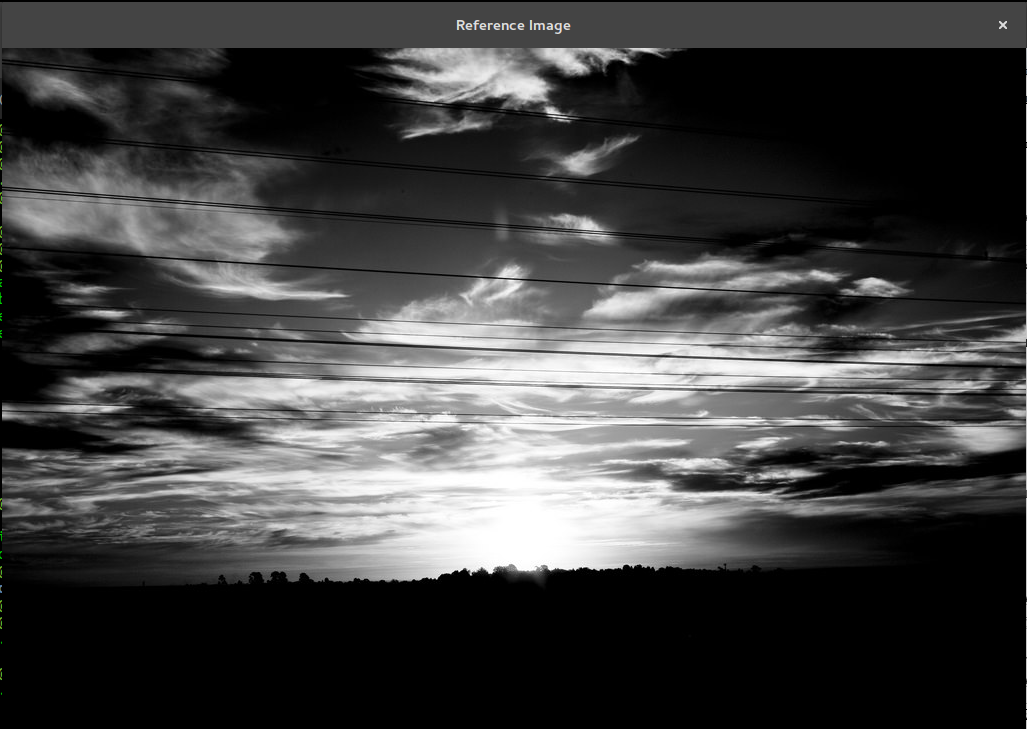
\includegraphics[scale=0.28]{../results/reference2.png}
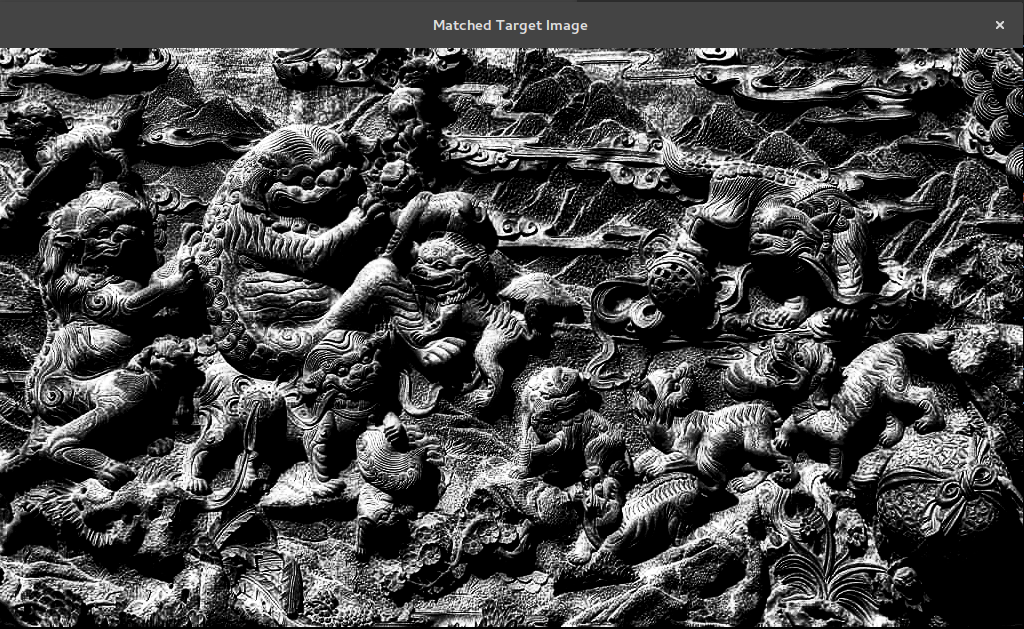
\includegraphics[scale=0.28]{../results/matched2.png}
\end{center}

\section*{Solution 3}
Let the 8-connect neighborhood of a point be given by
\begin{tabular}{| c | c | c |}
	\hline
	$v_{11}$	& $v_{12}$ 	& $v_{13}$ \\
	\hline
	$v_{21}$	& $v_{22}$ 	& $v_{23}$\\
	\hline
	$v_{31}$ 	& $v_{32}$  & $v_{33}$ \\
	\hline
\end{tabular}. \\ \\
In blinear interpolation, we fit a function $f(x, y)$ using weights $a_{ij}$ in the following manner :
\begin{align}
f(x, y) & = \Sigma_{i = 0}^1\Sigma_{j = 0}^1 a_{ij}x^i y^j
\end{align}
Let $x_1, x_2, x_3$ and $y_1, y_2, y_3$ be the x and y coordinates of the points in the neighborhood. It is clear that $x_1 \neq x_2$, $x_2 \neq x_3$, $x_3 \neq x_1$, $y_1 \neq y_2$, $y_2 \neq y_3$ and $y_3 \neq y_1$. Also, let $e$ be the error vector.
\begin{align}
We\ have,\ \begin{bmatrix}
				f(x_1, y_1) \\
				f(x_1, y_2) \\
				f(x_1, y_3) \\
				f(x_2, y_1) \\
				f(x_2, y_2) \\
				f(x_2, y_3) \\
				f(x_3, y_1) \\
				f(x_3, y_2) \\
				f(x_3, y_3)
			\end{bmatrix} & = 
			\begin{bmatrix}
				1 && x_1 &&	y_1 && x_1y_1 \\
				1 && x_1 &&	y_2 && x_1y_2 \\
				1 && x_1 &&	y_3 && x_1y_3 \\
				1 && x_2 &&	y_1 && x_2y_1 \\
				1 && x_2 &&	y_2 && x_2y_2 \\
				1 && x_2 &&	y_3 && x_2y_3 \\
				1 && x_3 &&	y_1 && x_3y_1 \\
				1 && x_3 &&	y_2 && x_3y_2 \\
				1 && x_3 &&	y_3 && x_3y_3 \\
			\end{bmatrix}
			\begin{bmatrix}
				a_{00} \\
				a_{01} \\
				a_{10} \\
				a_{11}	
			\end{bmatrix} + e \\
\implies\ \begin{bmatrix}
				v_{11} \\
				v_{12} \\
				v_{13} \\
				v_{21} \\
				v_{22} \\
				v_{23} \\
				v_{31} \\
				v_{32} \\
				v_{33}
			\end{bmatrix} & = 
			\begin{bmatrix}
				1 && x_1 &&	y_1 && x_1y_1 \\
				1 && x_1 &&	y_2 && x_1y_2 \\
				1 && x_1 &&	y_3 && x_1y_3 \\
				1 && x_2 &&	y_1 && x_2y_1 \\
				1 && x_2 &&	y_2 && x_2y_2 \\
				1 && x_2 &&	y_3 && x_2y_3 \\
				1 && x_3 &&	y_1 && x_3y_1 \\
				1 && x_3 &&	y_2 && x_3y_2 \\
				1 && x_3 &&	y_3 && x_3y_3 \\
			\end{bmatrix}
			\begin{bmatrix}
				a_{00} \\
				a_{01} \\
				a_{10} \\
				a_{11}	
			\end{bmatrix} + e
\end{align}
Our aim is to determine $\begin{bmatrix}
							a_{00} \\
							a_{01} \\
							a_{10} \\
							a_{11}	
						  \end{bmatrix}$ while minimizing the the MSE, $e^Te$. \\
Let $f = \begin{bmatrix}
				v_{11} \\
				v_{12} \\
				v_{13} \\
				v_{21} \\
				v_{22} \\
				v_{23} \\
				v_{31} \\
				v_{32} \\
				v_{33}
			\end{bmatrix}$,
    $X = \begin{bmatrix}
				1 && x_1 &&	y_1 && x_1y_1 \\
				1 && x_1 &&	y_2 && x_1y_2 \\
				1 && x_1 &&	y_3 && x_1y_3 \\
				1 && x_2 &&	y_1 && x_2y_1 \\
				1 && x_2 &&	y_2 && x_2y_2 \\
				1 && x_2 &&	y_3 && x_2y_3 \\
				1 && x_3 &&	y_1 && x_3y_1 \\
				1 && x_3 &&	y_2 && x_3y_2 \\
				1 && x_3 &&	y_3 && x_3y_3 \\
			\end{bmatrix}$ and
	$W = \begin{bmatrix}
			a_{00} \\
			a_{01} \\
			a_{10} \\
			a_{11}	
		 \end{bmatrix}$
\begin{align}
\therefore\ e & = f - XW
\end{align}
The best estimate for W is given by : 
\begin{align}
\hat{W} & = (X^TX)^{-1}X^Tf & on\ minimizing\ the\ MSE,\ e^Te.
\end{align}
We need $X^TX$ to be invertable for a solution to exist for the given interpolation problem.
Let us first show that $dim(nullspace\ of\ X) = 0$. We're going to prove that the column vectors of X are linearly independent, i.e. $c_1X_1 + c_2X_2 + c_3X_3 + c_4X_4 = 0\ \implies\ c_1 = c_2 = c_3 = c_4 = 0$ where $X = [X_1\ X_2\ X_3\ X_4]$ \\
On taking $c_1X_1 + c_2X_2 + c_3X_3 + c_4X_4 = 0$,
\begin{align}
We\ have,\ & c_1 + c_2x_1 + c_3y_1 + c_4x_1y_1 = 0 \\
& c_1 + c_2x_1 + c_3y_2 + c_4x_1y_2 = 0 \\
\implies\ & c_3(y_1 - y_2) + c_4x_1(y_1 - y_2) = 0\ & from\ (6) - (7) \\
\implies\ & (y_1 - y_2)(c_3 + c_4x_1) = 0 \\
\implies\ & c_3 + c_4x_1 = 0\ & \because\ y_1 \neq y_2 \\
Similiarly,\ using\ & c_1 + c_2x_2 + c_3y_1 + c_4x_2y_1 = 0 \\
& c_1 + c_2x_2 + c_3y_2 + c_4x_2y_2 = 0 \\
we\ get,\ & c_3 + c_4x_2 = 0 \\
\implies\ & c_3 = c_4 = 0\ & from\ (10),\ (13)\ and\ \because\ x_1 \neq x_2 \\  
Also, \ c_1 = c_2 = 0\ & from\ (6),\ (11),\ (14)\ and\ \because\ x_1 \neq x_2
\end{align}
$\therefore\ c_1X_1 + c_2X_2 + c_3X_3 + c_4X_4 = 0\ \implies\ c_1 = c_2 = c_3 = c_4 = 0$ \\
$\therefore\ dim(columnspace\ of\ X) = 4$ as the column vectors are linearly independent.
\begin{align}
Hence,\ dim(nullspace\ of\ X) = 4 - 4 = 0
\end{align}

We're now going to prove that $nullspace\ of\ X = nullspace\ of\ X^TX$.
\begin{align*}
Let\ y \in nullspace\ of\ X \\
\therefore\ & Xy = 0 \\
\implies\ & X^TXy = 0 \\
\implies\ & y \in nullspace\ of\ X^TX \\
\therefore\ & nullspace\ of\ X \subseteq\ nullspace\ of\ X^TX \\
\\
Let\ y \in nullspace\ of\ X^TX \\
\therefore\ & X^TXy = 0 \\
\implies\ & y^TX^TXy = 0 \\
\implies\ & (Xy)^TXy = 0 \\
\implies\ & Xy = 0 \\
\implies\ & y \in nullspace\ of\ X \\
\therefore\ & nullspace\ of\ X^TX \subseteq\ nullspace\ of\ X\
\end{align*}
\begin{align}
\therefore\ nullspace\ of\ X^TX = nullspace\ of\ X
\end{align}
Hence, $dim(nullspace\ of\ X^TX) = dim(nullspace\ of\ X) = 0$ using (17) and (18). \\
$X^TX$ is a $4\times4$ square matrix. It has full rank since its nullspace is 0. $\therefore\ X^TX$ is invertible and hence bilinear interpolation in an 8-neighborhood can always be used to get a solution for $W$ and (1) can be constructed. \\
The linear system is overdetermined, but it always has a rank of 4. Hence, an approximate solution can always be obtained through the pseudoinverse.

\pagebreak

\section*{Solution 4}
$\text{We are assuming that }\eta_i (x_1, y_1)\ and\ \eta_j (x_2, y_2)\text{ are independent if i }\neq j\ or\ x_1 \neq x_2\ or\ y_1 \neq y_2.$
\begin{align}
\therefore\ if\ i \neq j,\ E[\eta_i(x, y)\eta_j(x, y)] & = 0
\end{align}
\begin{align*}
We\ have,\ g_i(x, y) & = f_i(x, y) + \eta_i(x, y) \\
Also,\ f_i(x, y) & = f(x, y) \\
Now,\ \hat{g}(x, y)& = \frac{1}{K} \Sigma_{i = 1}^K g_i(x, y) \\
& = \frac{1}{K}K f(x, y) + \frac{1}{K}\Sigma_{i = 1}^K \eta_i(x, y) \\
& = f(x, y) + \frac{1}{K}\Sigma_{i = 1}^K \eta_i(x, y) \\
Now,\ noise\ variance,\ E[(\hat{g}(x, y) - f(x, y))^2] & = E[(\frac{1}{K}\Sigma_{i = 1}^K \eta_i(x, y))^2] \\
& = \frac{1}{K^2}\Sigma_{i = 1}^K\Sigma_{j = 1}^K E[\eta_i(x, y)\eta_j(x, y)] \\
& = \frac{1}{K^2}\Sigma_{i = 1}^K E[\eta_i(x, y)^2] & from\ (18) \\
& = \frac{1}{K^2}\Sigma_{i = 1}^K \sigma^2 & \because\ E[\eta_i(x, y)^2] = \sigma^2 \\
& = \frac{\sigma^2}{K} \\
q.e.d
\end{align*}

\section*{Solution 5}

Let $f(x, y, z) : \Re^3 \rightarrow \Re$. Let $[u\ v\ w]^T$ be the position of $[x\ y\ z]^T$ in a rotated cooridnate frame.
The relationship between $[u\ v\ w]^T$ and $[x\ y\ z]^T$ is given by :
\begin{align}
\begin{bmatrix}
	u \\
	v \\
	w
\end{bmatrix} & =
	R
\begin{bmatrix}
	x \\
	y \\
	z
\end{bmatrix} \\
where,\ R & = [R_1\ R_2\ R_3] \\
& = \begin{bmatrix}
		R_{11} & R_{12} & R_{13} \\
		R_{21} & R_{22} & R_{23} \\
		R_{31} & R_{32} & R_{33}
	\end{bmatrix} \\
Known\ properties\ of\ R,\ |R_1| & = 1 \\
|R_2| & = 1 \\
R_1^T R_2 & = 0 \\
R_3  & = R_1 \times R_2 \\
\implies\ |R_3| & = 1 \\
R_1^T R_3 & = R_2^T R_3 = 0 \\
R^{-1} & = R^T \\
We\ can\ also\ write,\
\begin{bmatrix}
	x \\
	y \\
	z
\end{bmatrix} & =
	R^T
\begin{bmatrix}
	u \\
	v \\
	w
\end{bmatrix} & from\ (19),\ (28)
\end{align}
\begin{align}
Now,\ \frac{\partial f}{\partial u} & =
\frac{\partial f}{\partial x}\frac{\partial x}{\partial u} +
\frac{\partial f}{\partial y}\frac{\partial y}{\partial u} +
\frac{\partial f}{\partial z}\frac{\partial z}{\partial u} \\
& = R_{11}\frac{\partial f}{\partial x} +
	R_{12}\frac{\partial f}{\partial y} +
	R_{13}\frac{\partial f}{\partial z} & from\ (21), (29) \\
Similarily,\ \frac{\partial f}{\partial v}
& = R_{21}\frac{\partial f}{\partial x} +
	R_{22}\frac{\partial f}{\partial y} +
	R_{23}\frac{\partial f}{\partial z}\\
\ \frac{\partial f}{\partial w}
& = R_{31}\frac{\partial f}{\partial x} +
	R_{32}\frac{\partial f}{\partial y} +
	R_{33}\frac{\partial f}{\partial z}
\end{align}
\begin{align}
\therefore\ \frac{\partial^2 f}{\partial^2 u} & =
R_{11}
(\frac{\partial^2 f}{\partial^2 x} \frac{\partial x}{\partial u} +
 \frac{\partial^2 f}{\partial y \partial x} \frac{\partial y}{\partial u} +
 \frac{\partial^2 f}{\partial z \partial x} \frac{\partial z}{\partial u})\notag \\
& + R_{12}(\frac{\partial^2 f}{\partial x \partial y} \frac{\partial x}{\partial u}
  + \frac{\partial^2 f}{\partial^2 y} \frac{\partial y}{\partial u}
  +	 \frac{\partial^2 f}{\partial z \partial x} \frac{\partial z}{\partial u}) \notag \\
& + R_{13}(\frac{\partial^2 f}{\partial x \partial z} \frac{\partial x}{\partial u}
  + \frac{\partial^2 f}{\partial y \partial z} \frac{\partial y}{\partial u} 
  +	 \frac{\partial^2 f}{\partial^2 z} \frac{\partial z}{\partial u}) & from\ (31)\ and\ chain\ rule \\
& = R_{11}^2\frac{\partial^2 f}{\partial^2 x} +
	R_{11}R_{12}\frac{\partial^2 f}{\partial y \partial x} +
	R_{11}R_{13}\frac{\partial^2 f}{\partial z \partial x}\notag \\
& + R_{12}R_{11}\frac{\partial^2 f}{\partial x \partial y} +
	R_{12}^2\frac{\partial^2 f}{\partial^2 y} +
	R_{12}R_{13}\frac{\partial^2 f}{\partial z \partial y}\notag \\
& + R_{13}R_{11}\frac{\partial^2 f}{\partial x \partial z} +
	R_{13}R_{12}\frac{\partial^2 f}{\partial y \partial z} +
	R_{13}^2\frac{\partial^2 f}{\partial^2 z} & from\ (21), (29) \\
Similarily,\ \frac{\partial^2 f}{\partial^2 v} & =
	R_{21}^2\frac{\partial^2 f}{\partial^2 x} +
	R_{21}R_{22}\frac{\partial^2 f}{\partial y \partial x} +
	R_{21}R_{23}\frac{\partial^2 f}{\partial z \partial x}\notag \\
& + R_{22}R_{21}\frac{\partial^2 f}{\partial x \partial y} +
	R_{22}^2\frac{\partial^2 f}{\partial^2 y} +
	R_{22}R_{23}\frac{\partial^2 f}{\partial z \partial y}\notag \\
& + R_{23}R_{21}\frac{\partial^2 f}{\partial x \partial z} +
	R_{23}R_{22}\frac{\partial^2 f}{\partial y \partial z} +
	R_{23}^2\frac{\partial^2 f}{\partial^2 z} \\
\frac{\partial^2 f}{\partial^2 w} & =
	R_{31}^2\frac{\partial^2 f}{\partial^2 x} +
	R_{31}R_{32}\frac{\partial^2 f}{\partial y \partial x} +
	R_{31}R_{33}\frac{\partial^2 f}{\partial z \partial x}\notag \\
& + R_{32}R_{31}\frac{\partial^2 f}{\partial x \partial y} +
	R_{32}^2\frac{\partial^2 f}{\partial^2 y} +
	R_{32}R_{33}\frac{\partial^2 f}{\partial z \partial y}\notag \\
& + R_{33}R_{31}\frac{\partial^2 f}{\partial x \partial z} +
	R_{33}R_{32}\frac{\partial^2 f}{\partial y \partial z} +
	R_{33}^2\frac{\partial^2 f}{\partial^2 z}
\end{align}
On performing $(35) + (36) + (37)$, we get using (22), (23), (24), (26) and (27)
\begin{align}
\frac{\partial^2 f}{\partial^2 u} +
\frac{\partial^2 f}{\partial^2 v} +
\frac{\partial^2 f}{\partial^2 w} & =
\frac{\partial^2 f}{\partial^2 x} +
\frac{\partial^2 f}{\partial^2 y} +
\frac{\partial^2 f}{\partial^2 z}\\
\implies\ \nabla^2 f(u, v, w) & = \frac{\partial^2 f}{\partial^2 u} +
							  \frac{\partial^2 f}{\partial^2 v} +
						      \frac{\partial^2 f}{\partial^2 w} \\
						      & = \frac{\partial^2 f}{\partial^2 x} +
							  \frac{\partial^2 f}{\partial^2 y} +
						      \frac{\partial^2 f}{\partial^2 z} & from\ (38) \\
						      & =  \nabla^2 f(x, y, z) \\
\implies & Laplacian\ (\nabla^2)\ is\ isotropic\ (rotation\ invariant). \notag
\end{align}

\section*{Solution 6}
A C++ file, Q6/src/Q6.cxx, contains the code required to perform the required task.

In order to build and run the code, the following steps need to be followed :
\begin{enumerate}
\item Enter Q6/src through terminal.
\item run build.sh (OpenCV needs to installed and a version of g++ supporting c++14 needs to be present)
\item Execute Q6 (the binary file) with the relative/absolute image path. Eg. [./Q6 ../../images/divyat.jpg] or [./Q6 ../../images/low.jpg] (On Ubuntu)
\item The program can be closed by Ctrl+C on the terminal or by pressing `q' when one of the image windows is open.
\end{enumerate}
\pagebreak
\subsection*{Results}
\begin{center}
divyat.jpg \\
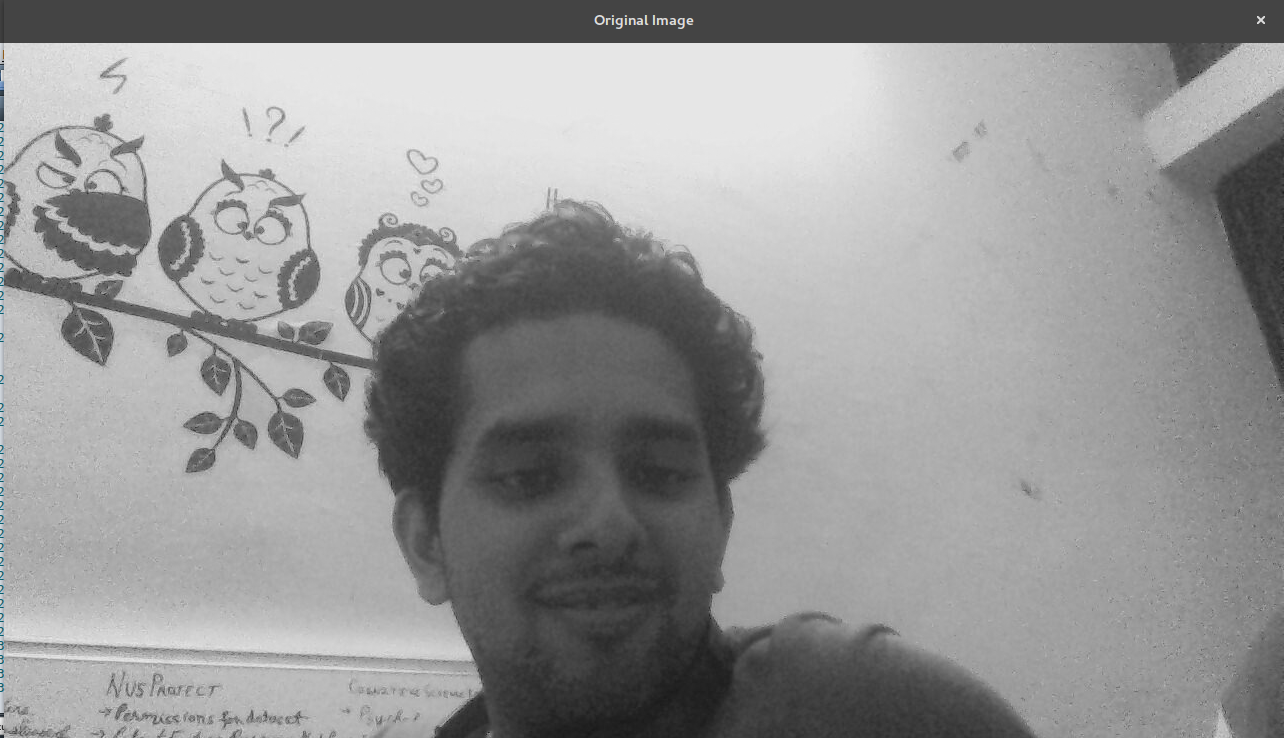
\includegraphics[scale= 0.24]{../results/divyat.png}
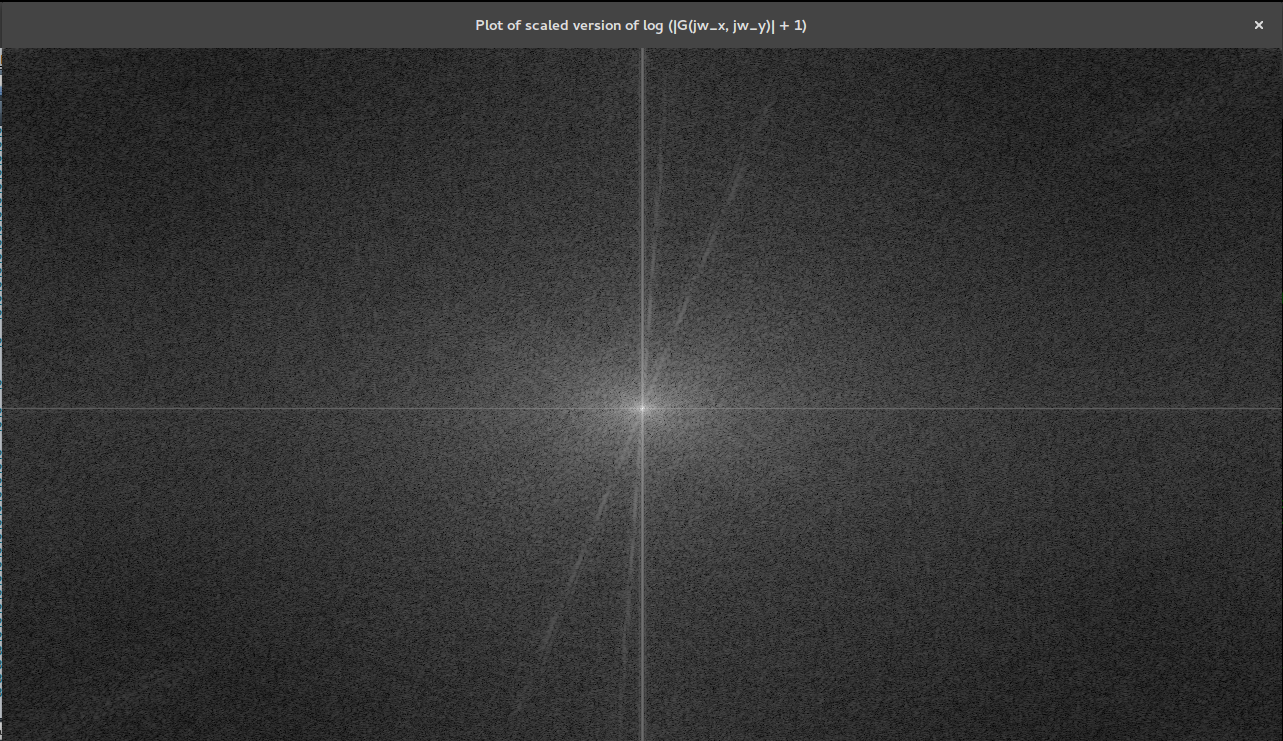
\includegraphics[scale= 0.24]{../results/divyat_spectrum.png}
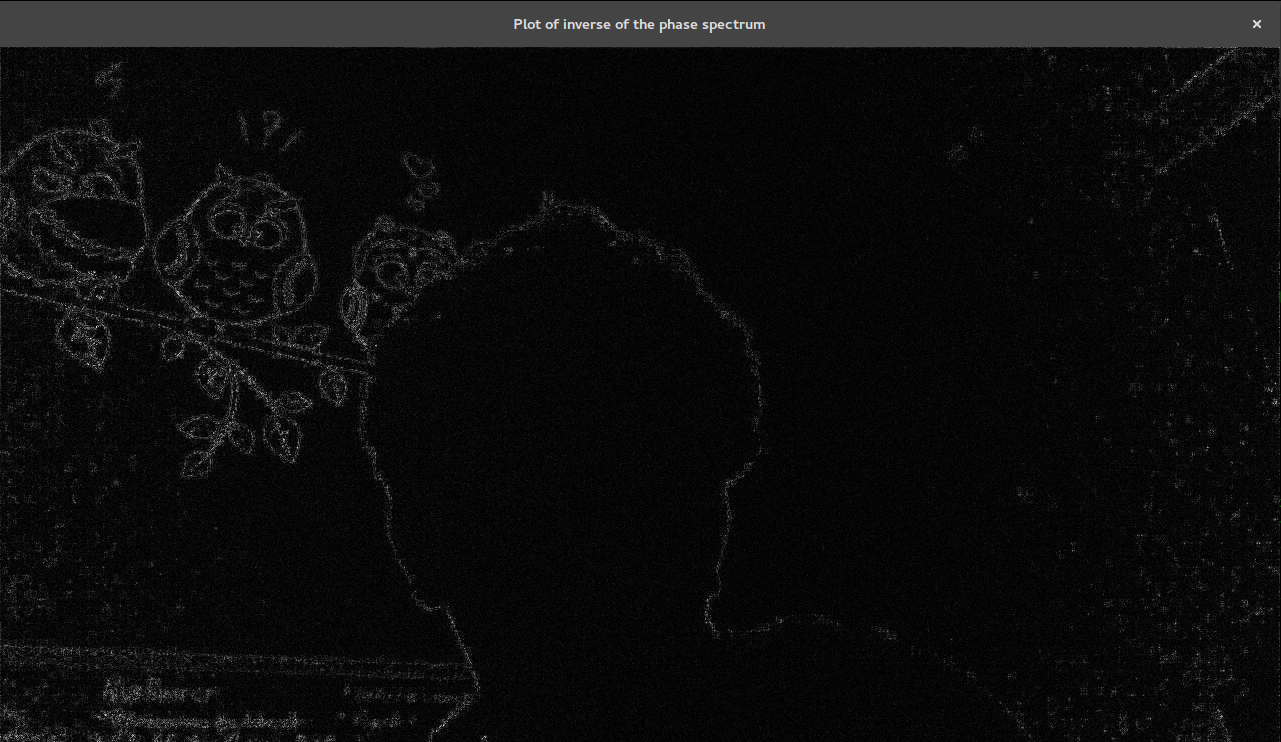
\includegraphics[scale= 0.24]{../results/divyat_phase.png}
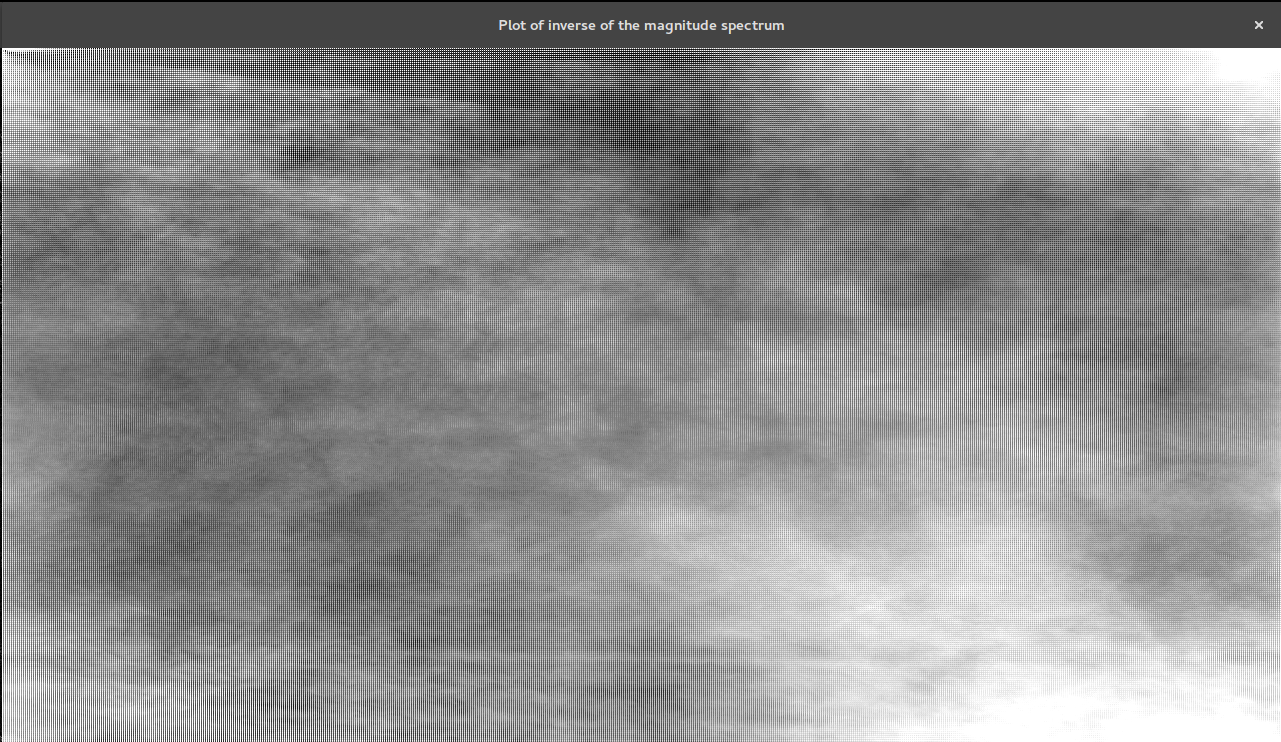
\includegraphics[scale= 0.24]{../results/divyat_magnitude.png}
\end{center}
\pagebreak
\begin{center}
low.jpg \\
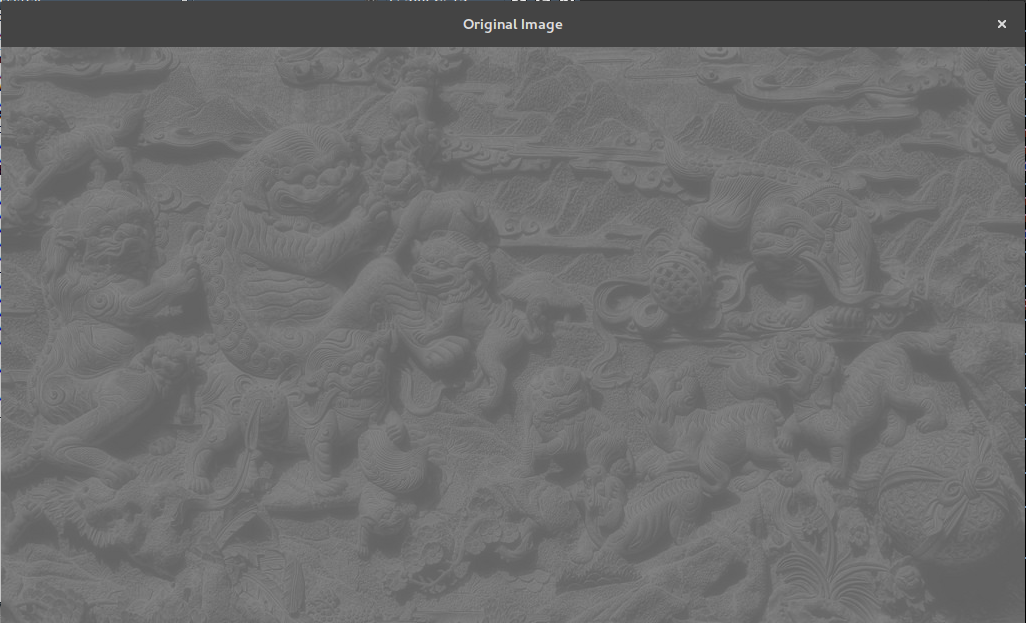
\includegraphics[scale= 0.29]{../results/low.png}
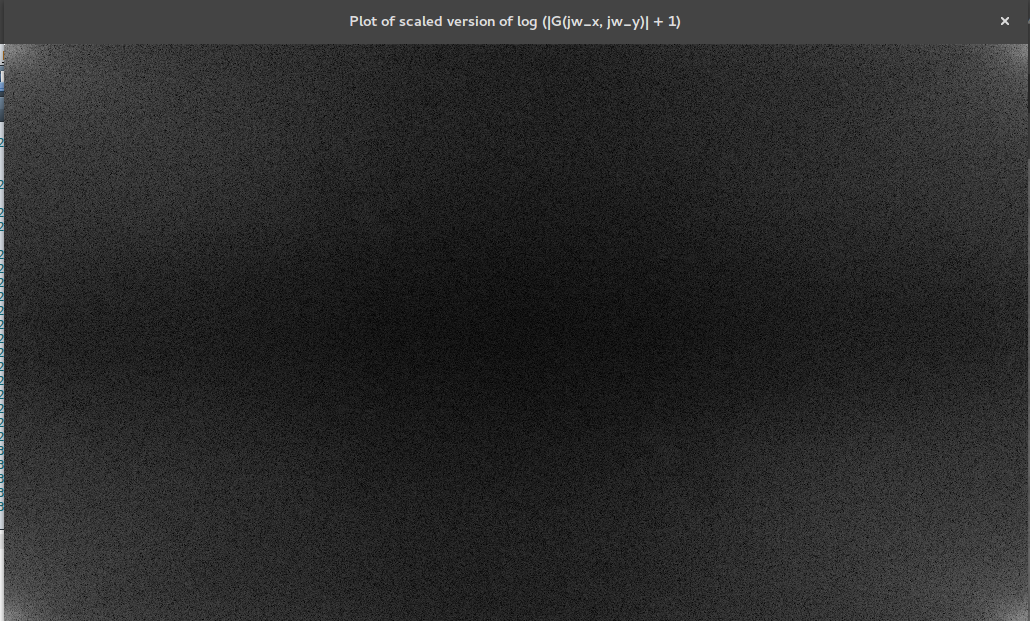
\includegraphics[scale= 0.29]{../results/low_spectrum.png}
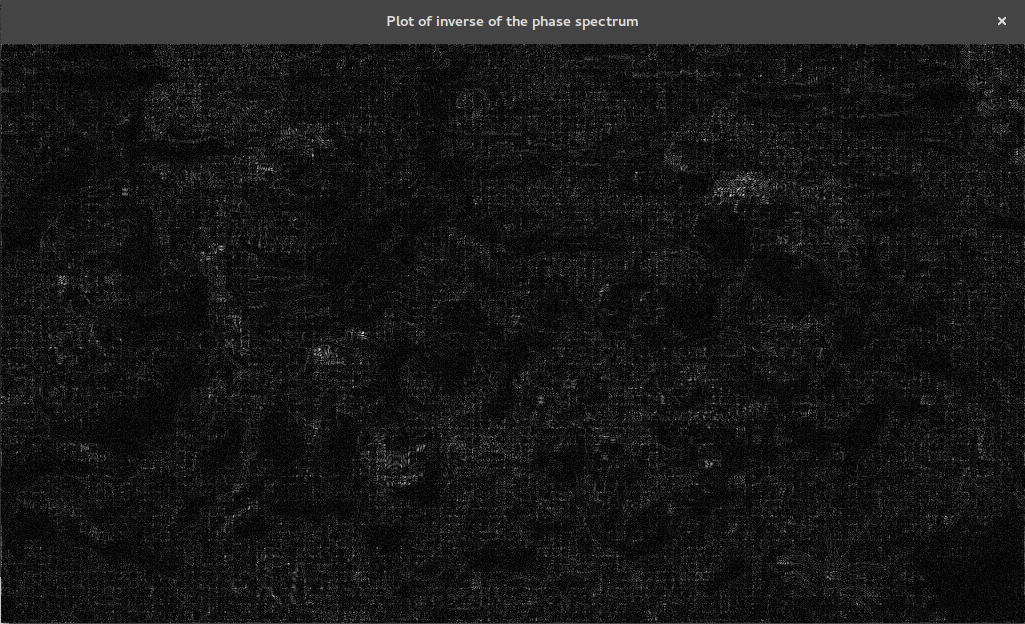
\includegraphics[scale= 0.29]{../results/low_phase.png}
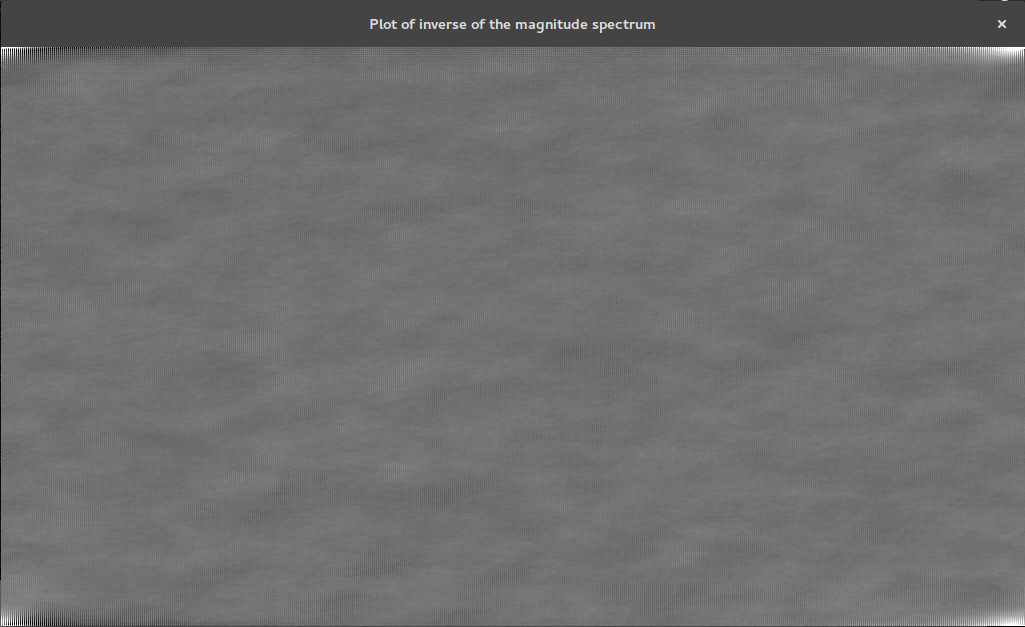
\includegraphics[scale= 0.29]{../results/low_magnitude.png}
\end{center}
\subsection*{Observations}
\subsubsection*{Reconstruction using only phase spectrum}
From the above the tests, it can be inferred that on performing reconstruction using only phase information, edges are being preserved and we are losing all the grey-levels of homogenous regions. From the spectrum plots, we can infer that the lower frequency components tend to have greater values than the higher frequency ones in general images. Thus, when we remove the magnitude information, the lower frequency components are getting more suppressed than the higer frequency components, i.e. the operation is similar to a high-pass filter. This premise explains the above images obatined using only the phase spectrum.
\subsubsection*{Reconstruction using only magnitude spectrum}
The reconstruction using only magnitude spectrum appears to only contain information regarding the prominent greylevels present in the image.

\section*{Solution 7}
Code has been written in two .cxx files :
\begin{enumerate}
\item Q7/src/pixel\_nlm.cxx : Contains the function, EE604A::pixel\_nlm(), used to perform neighborhood filter using non-local pixel values.
\item Q7/src/Q7.cxx : Calls the contained function, task(), which adds noise as needed and evaluated the neighborhood filtering method.
\end{enumerate}

There is also a header file present for the EE604A::pixel\_nlm() function :
\begin{enumerate}
\item Q7/include/pixel\_nlm.cxx
\end{enumerate}

In order to build and run the code, the following steps need to be followed :
\begin{enumerate}
\item Enter Q7/src through terminal.
\item run build.sh (OpenCV needs to installed and a version of g++ supporting c++14 needs to be present)
\item Execute Q7 (the binary file) with the relative/absolute image path. Eg. [./Q7 ../../images/small.jpg] (On Ubuntu)
\item The program can be closed by Ctrl+C on the terminal or by pressing `q' when one of the image windows is open.
\end{enumerate}
\begin{center}
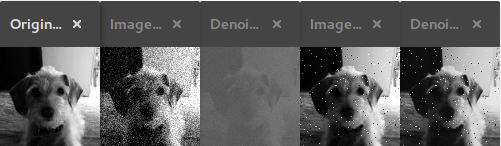
\includegraphics[scale=1.0]{../results/Q7.png}
\end{center}
The images from left to right are as follows : (a) The original image (small.jpg), (b) The images with added zero-mean gaussian noise with $\sigma^2 = 0.01$, (c) The reconstucted image [b], (d) The image with impulse noise, (e) The reconstructed image [d]
\end{document}